%!TEX root = SISC_elastic_3d.tex
\subsection{Energy conservation test}\label{conserved_energy}
To verify the energy conservation property of our scheme, we perform computation without external source term, but with a Gaussian initial profile  centered at the origin of the computational domain.  Specifically, the computational domain, density function $\rho$ and material functions $\mu, \lambda$ are taken to be the same as in the Section \ref{convergence_study}; the initial Gaussian profile is
\begin{align*}
	u_1(\cdot,0) &= \mbox{exp}\left(-\frac{(x^{(1)}-\pi)^2}{0.1}\right)\mbox{exp}\left(-\frac{(x^{(2)}-\pi)^2}{0.1}\right)\mbox{exp}\left(-\frac{(x^{(3)}-\pi)^2}{0.1}\right),\\
	u_2(\cdot,0) &= \mbox{exp}\left(-\frac{(x^{(1)}-\pi)^2}{0.2}\right)\mbox{exp}\left(-\frac{(x^{(2)}-\pi)^2}{0.2}\right)\mbox{exp}\left(-\frac{(x^{(3)}-\pi)^2}{0.2}\right),\\
	u_3(\cdot,0) &= \mbox{exp}\left(-\frac{(x^{(1)}-\pi)^2}{0.1}\right)\mbox{exp}\left(-\frac{(x^{(2)}-\pi)^2}{0.2}\right)\mbox{exp}\left(-\frac{(x^{(3)}-\pi)^2}{0.2}\right).
\end{align*}
 The grid spacing in the parameter space for coarse domain $\Omega^c$ is $2h_1 = 2h_2 = 2h_3 = \frac{\pi}{24}$ and for fine domain $\Omega^f$ is $h_1 = h_2 = h_3 = \frac{\pi}{48}$. Thus we have $25\times25\times13$ grid points in the coarse domain $\Omega^c$ and $49\times49\times25$ grid points in the fine domain $\Omega^f$. 

For the semi-discrete approximation, the energy is given by $({\bf F}_t,{\rho}^f{\bf F}_t)_h + \mathcal{S}_h({\bf F},{\bf F}) + ({\bf C}_t,{\rho}^{c}{\bf C}_t)_{2h} + \mathcal{S}_{2h}({\bf C},{\bf C})$, see (\ref{semi_energy_1}). By using the same approach as for the isotropic elastic wave equation, see \cite{petersson2015wave,sjogreen2012fourth},  the expression for the fully discrete energy reads as
\begin{align*}
E^{n+1/2} &= \left|\left|\sqrt{{\rho}^f}\frac{{\bf F}^{n+1}-{\bf F}^n}{\Delta t}\right|\right|_h^2 + S_h({\bf F}^{n+1},{\bf F}^n) - \frac{(\Delta t)^2}{12}((J^f)^{-1}\mathcal{L}^h{\bf F}^{n+1},(J^f)^{-1}\mathcal{L}^h{\bf F}^n)_h\\
&+ \left|\left|\sqrt{{\rho}^{c}}\frac{{\bf C}^{n+1}-{\bf C}^n}{\Delta t}\right|\right|_{2h}^2 + S_{2h}({\bf C}^{n+1},{\bf C}^n) - \frac{(\Delta t)^2}{12}((J^c)^{-1}\wt{\mathcal{L}}^{2h}{\bf C}^{n+1},(J^c)^{-1}\wt{\mathcal{L}}^{2h}{\bf C}^n)_{2h}.
\end{align*}
We present the relative change in fully discrete energy, $(E^{n+1/2}-E^{1/2})/E^{1/2}$, as a function of time with $t\in[0,90]$ in Figure \ref{discrete_energy}. This corresponds to $6186$ time steps. Our numerical results show that the fully discrete energy remains constant up to round-off error.
\begin{figure}[htbp]
	\centering
	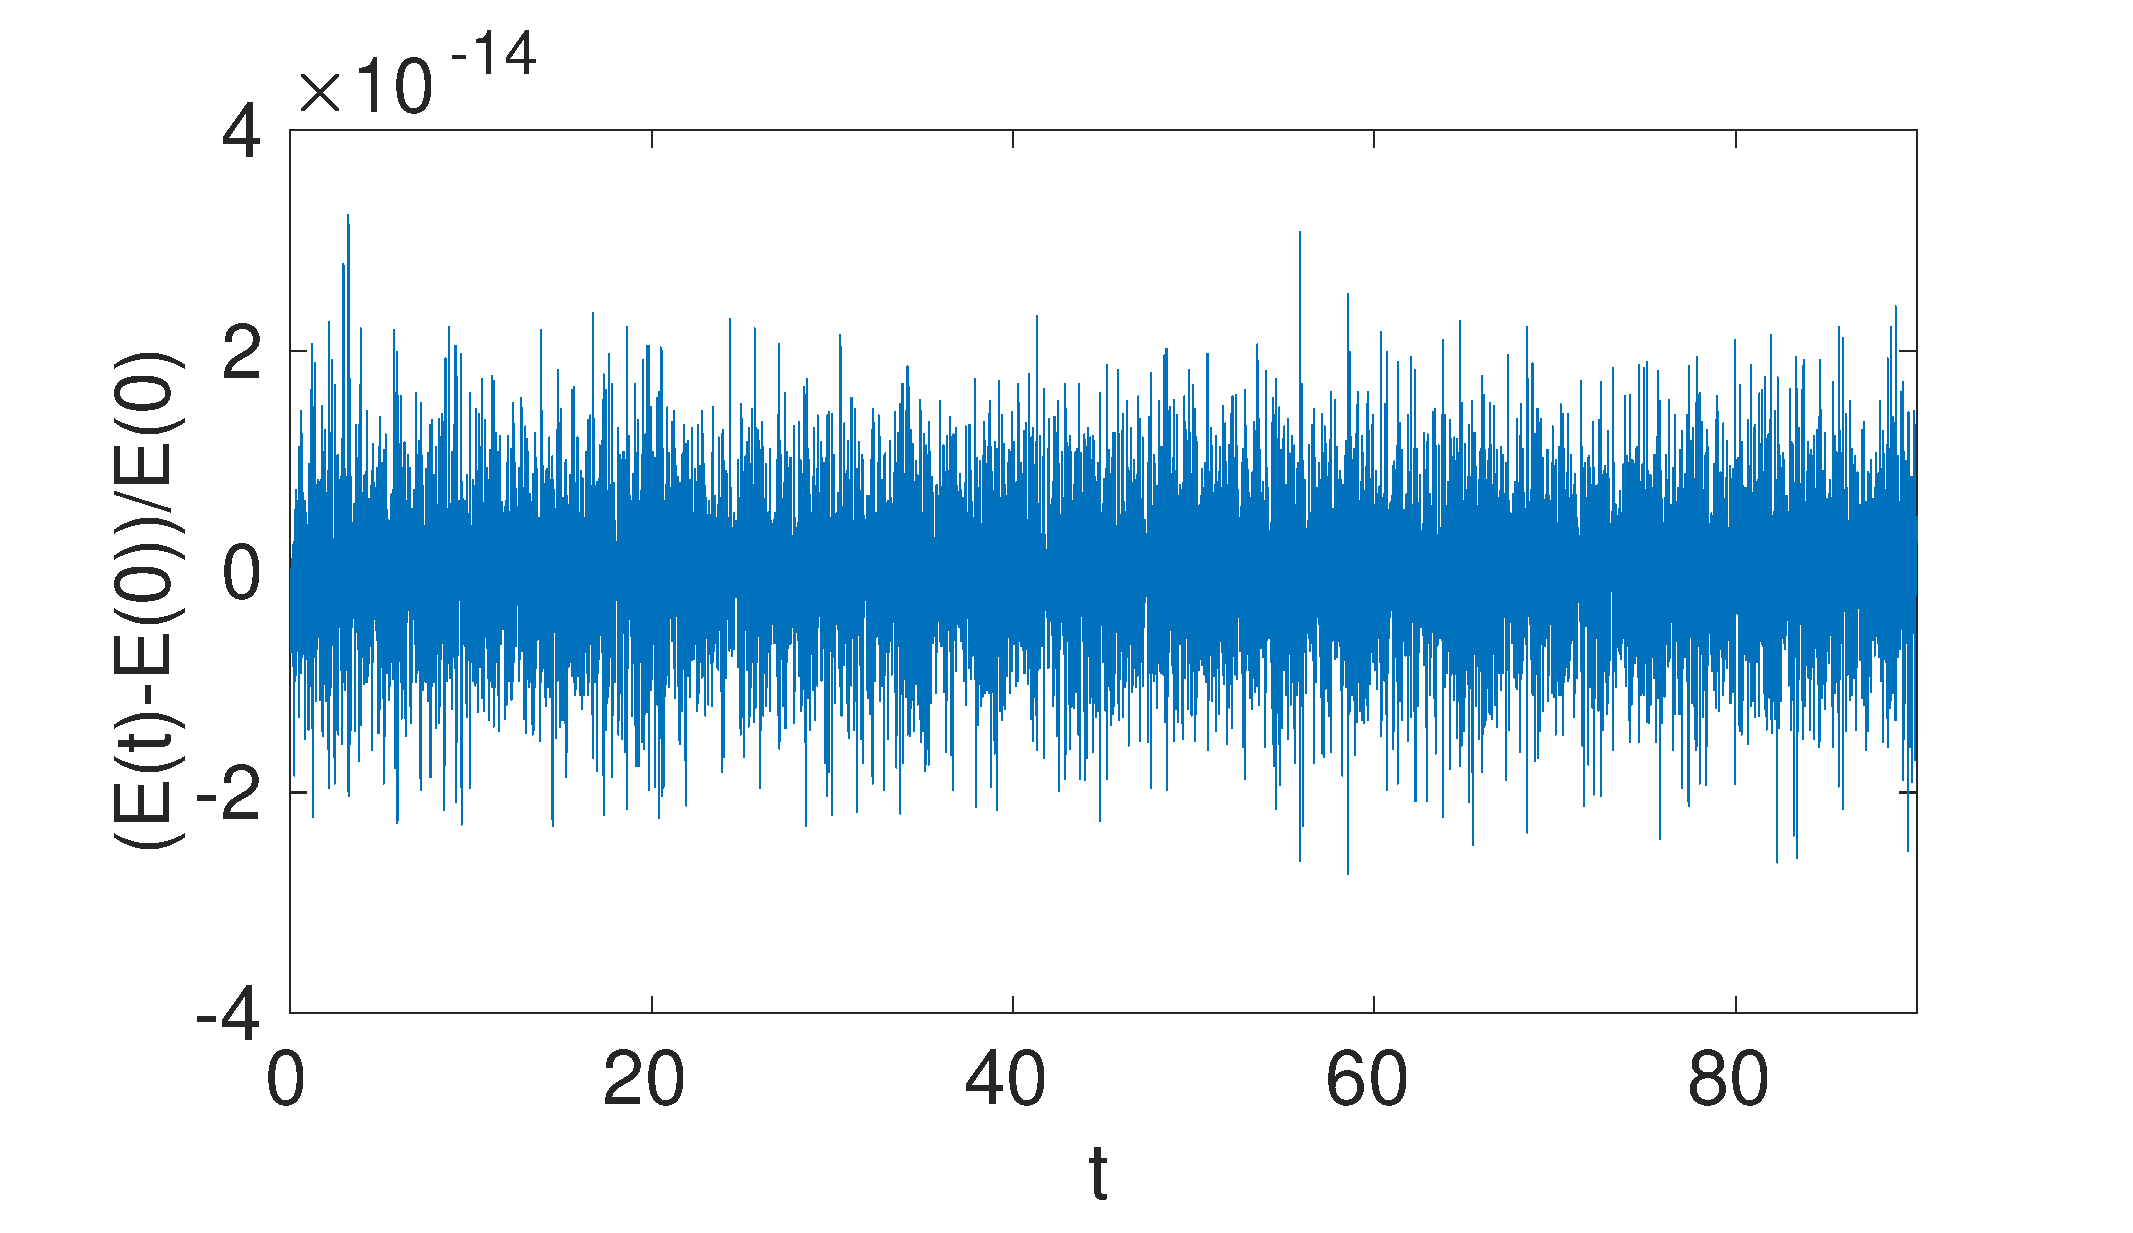
\includegraphics[width=0.6\textwidth,trim={0cm 0cm 0cm 0cm}, clip]{discrete_energy.eps}
	\caption{The relative change in fully discrete energy as a function of time. Here, $t = 90$ corresponds to $6186$ time steps.}\label{discrete_energy}
\end{figure}


